\subsection{Relace ekvivalence}
\label{ssec:relace-ekvivalence}

Ekvivalence je relací na množině, která umožňuje dělit ji na části tvořené ve
smyslu daném touto relací \uv{stejnými}/ekvivalentními prvky. Ačkolivěk formálně
nemá \emph{relace} ekvivalence nic společného s \emph{logickou operací}
ekvivalence, důvody pro jejich jména souhlasí. Totiž, \emph{logická} ekvivalence
spojuje dva výroky, které jsou v pravdivostním smyslu stejné, a \emph{relační}
ekvivalence spojuje dva prvky množiny, které rovněž chceme (v daném kontextu)
považovat za totožné.

\begin{definition}{Relace ekvivalence}{relace-ekvivalence}
 Relaci $R$ na množině $A$ nazveme \emph{ekvivalencí}, pokud je
 \begin{itemize}
  \item reflexivní ($ \forall x \in A:xRx$),
  \item symetrická ($ \forall x,y \in A:xRy \Rightarrow yRx$),
  \item transitivní ($ \forall x,y,z \in A:(xRy \wedge yRz) \Rightarrow xRz$).
 \end{itemize}
\end{definition}
Spěšně si rozmyslíme smysluplnost této definice. Řekněme, že zkoumáme určité
vlastnosti lidí v~závislosti na jejich věku. Při takovéto studii pochopitelně
uvažujeme o dvou různých lidech stejného věku jako o \uv{totožných} subjektech.
Je samozřejmé, že dva skutečně stejné lidi považujeme za totožné (to vysvětluje
\emph{reflexivitu}). Podobně, když je člověk \emph{Jáchym} stejně starý jako
člověk \emph{Eric}, pak je i \emph{Eric} stejně starý jako \emph{Jáchym} (to
vysvětluje \emph{symetrii}). Konečně, když je člověk \emph{Lenin} stejně starý
jako člověk \emph{Stalin} a \emph{Stalin} je stejně starý jako \emph{Trotsky},
pak je přirozeně \emph{Lenin} stejně starý jako \emph{Trotsky} (to vysvětluje
\emph{transitivitu}).

Díky relaci \uv{býti stejného věku} můžeme nyní rozdělit množinu všech lidí na
Zemi na 122 (nejstarší zaznamenaný lidský věk) chlívků; v každém chlívku všichni
lidé stejně staří. Těmto \uv{chlívkům} se v matematice přezdívá \emph{třídy
ekvivalence}. Třídy ekvivalence $R$ na množině $A$ jsou podmnožiny $A$, kde
v~každé podmnožině jsou přesně jen ty prvky, které jsou spolu v relaci $R$.

\begin{definition}{Třída ekvivalence}{trida-ekvivalence}
 Ať $A$ je množina a $R$ ekvivalence na $A$. Vezměme $x \in A$. \emph{Třídou
 ekvivalence} prvku $x$ podle $R$, zapsanou $[x]_R$, myslíme množinu
 \[
  [x]_R \coloneqq \{y \in A \mid xRy\}
 \]
 všech prvků $y \in A$ v relaci $R$ s $x$. O podmnožině $X \subseteq A$ řekneme,
 že je to \emph{třída ekvivalence} $A$ podle $R$, když existuje prvek $x \in A$
 takový, že $X = [x]_R$.
\end{definition}

Jak lze snadno vyčíst z příkladu studie vlastností lidí stejného věku, každý
člověk je v právě jednom chlívku/třídě ekvivalence (jednomu člověku nemůže být
různý počet let, metabolický věk ignorujeme) a navíc každý člověk je nutně v
některém. Vladouce jazykem matematiky řčeme, že třídy ekvivalence dvou prvků
jsou buď stejné (oba lidé v témž chlívku), nebo disjunktní (každý člověk
v~různém chlívku). Navíc, sjednocením všech tříd ekvivalence dostaneme původní
množinu $A$, stejně jako spojením všech chlívků dostaneme jeden velký chlév s
batolaty i kmety na jedné hromadě. Tento fakt je platný pro každou ekvivalenci a
je oním klíčovým důvodem užitečnosti tohoto konceptu.

\begin{proposition}{O třídách ekvivalence}{o-tridach-ekvivalence}
 Ať $R$ je ekvivalence na $A$ a $X,Y$ jsou třídy ekvivalence $A$ podle $R$. Pak
 buď $X = Y$, nebo $X \cap Y = \emptyset$. Navíc, je-li 
 \[
  \mathcal{X} \coloneqq \{X \subseteq A\mid X \text{ třída ekvivalence } A
  \text{ podle } R\}
 \]
 množina všech (podle předchozí věty navzájem disjunktních) tříd ekvivalence
 množiny $A$ podle $R$, pak
 \[
  A = \bigcup \mathcal{X}.
 \]
\end{proposition}

Pro nějaký číselný příklad relace ekvivalence -- jenž zároveň ukazuje, že tříd
ekvivalence nemusí být konečně mnoho -- uvažme třeba relaci \uv{býti mocninou}
na přirozených číslech. Řekneme, že číslo $n \in \N$ je \emph{mocninou} $m \in
N$, když existuje kladné \textbf{racionální} (abychom mohli uvažovat i
odmocniny) číslo $q$ takové, že $n = m^{q}$. Taková relace je jistě ekvivalence,
neboť
\begin{itemize}
 \item $ \forall n \in \N: n = n^{1}$, tedy každé číslo je svou vlastní
  mocninou (reflexivita);
 \item když $n = m^{q}$, pak $m = n^{\frac{1}{q}}$, čili předpoklad, že $n$ je
  mocninou $m$, implikuje, že $m$ je mocninou $n$ (symetrie);
 \item když $n = m^{q_1}$ a $m = l^{q_2}$, pak $n = l^{q_1q_2}$, čili pokud je
  $n$ mocninou $m$ a $m$ mocninou $l$, pak $n$ je mocninou $l$ (transitivita).
\end{itemize}

\myref{Obrázek}{fig:tridy-ekvivalence-mocniny} zobrazuje prvních několik tříd
ekvivalence \uv{býti mocninou} na množině přirozených čísel.

\begin{figure}[ht]
 \centering
 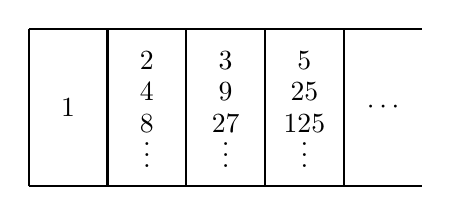
\begin{tikzpicture}
  \foreach \x in {0,1,2,3,4} {
    \draw[thick] (\x,0) -- (\x+1,0);
    \draw[thick] (\x,2) -- (\x+1,2);
    \draw[thick] (\x,0) -- (\x,2);
  }
  \node at (0.5,1) {$1$};

  \node at (1.5,1.6) {$2$};
  \node at (1.5,1.2) {$4$};
  \node at (1.5,0.8) {$8$};
  \node at (1.5,0.5) {$\vdots$};

  \node at (2.5,1.6) {$3$};
  \node at (2.5,1.2) {$9$};
  \node at (2.5,0.8) {$27$};
  \node at (2.5,0.5) {$\vdots$};
  
  \node at (3.5,1.6) {$5$};
  \node at (3.5,1.2) {$25$};
  \node at (3.5,0.8) {$125$};
  \node at (3.5,0.5) {$\vdots$};

  \node at (4.5,1) {$\cdots$};
  
 \end{tikzpicture}

 \caption{Třídy ekvivalence \uv{býti mocninou} na $\N$.}
 \label{fig:tridy-ekvivalence-mocniny}
\end{figure}
